\subsection{RAM access time}

\subsection{RAM bandwidth}



\subsection{Page Fault Service Time}

To profile page faults, we have used a mechanism proper to the Linux operating system called \textbf{Cgroups}. Cgroups are "tags" which can be specified when running process and which indicate to the operating system that only a restricted set of resources (indicated in the Cgroup description) should be allocated to the process. For example, we have restricted the amount of RAM used by the process for this experiment to 75MB.

In the experiment, we proceed to allocate an array (called \texttt{mallocs}) of 150 strings, each 1MB long. In order to ensure that the memory is actually allocated, we fill these 1MB strings with actual data. The memory allocation is done sequentially (the string for \texttt{mallocs[0]} is constructed before the string for \texttt{mallocs[1]} and so on...).

\begin{figure}
 \centering
  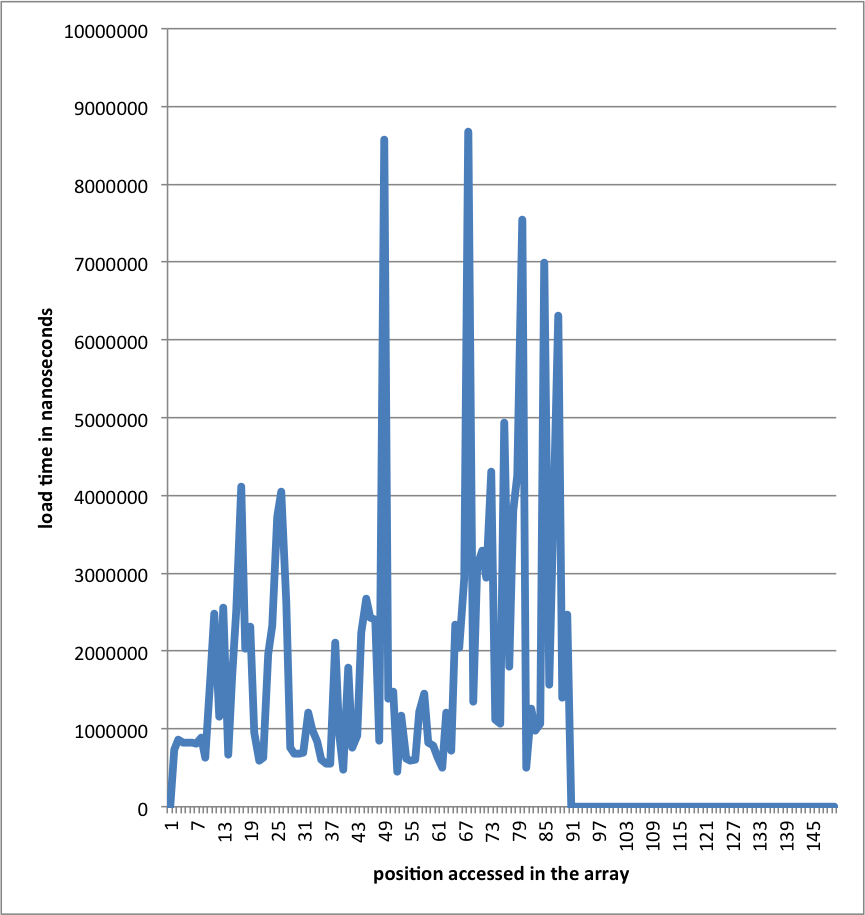
\includegraphics[width=0.5\textwidth]{image/pagefault.png}
  \caption{Page faults when accessing 150MB array}
 \label{fig:pagefault}
\end{figure}

Given the process can only 75MB of RAM, we can expect that at least half of the pages used by the \texttt{mallocs} array have been flushed to disk. Given data has been allocated sequentially, we can expect (according to the LRU rule), that these pages correspond to the first half of the array.

These expectations are confirmed on figure ~\ref{fig:pagefault}. In this figure, we measure the time required to load each of the 1MB strings sequentially using \texttt{memcpy()} (we start by loading \texttt{mallocs[0]} and finish with \texttt{mallocs[149]}. 
Given that the page size of our system is 4KB, 1MB corresponds to 256 pages. The average page load time for the first 90 MB is 1928/256 = 7.53  microseconds (which is consistent with the 750MB/sec bandwidth of our SSD). On the other hand, the average page load time for the last 60 MB is 1.1/256 = 0.00431  microseconds. This corresponds to a 2000x increase when fetching pages from disk rather than main memory!